%%%%%%%%%%%%%%%%%%%%%%%%%%%%%%%%%%%%%%%%%%%%%%%%%%%%%%%%%%%%%



%%%%%%%%%%%%%%%%%%%%%%%%%%%%%%%%%%%%%%%%%%%%%%%%%%%%%%%%%%%%%

%% HEADER

%%%%%%%%%%%%%%%%%%%%%%%%%%%%%%%%%%%%%%%%%%%%%%%%%%%%%%%%%%%%%

\documentclass[a4paper,twoside,10pt]{report}

% Alternative Options:

% Paper Size: a4paper / a5paper / b5paper / letterpaper / legalpaper /
% executivepaper

% Duplex: oneside / twoside

% Base Font Size: 10pt / 11pt / 12pt





%% Language %%%%%%%%%%%%%%%%%%%%%%%%%%%%%%%%%%%%%%%%%%%%%%%%%

\usepackage[USenglish]{babel} %francais, polish, spanish, ...

\usepackage[T1]{fontenc}

\usepackage[ansinew]{inputenc}



\usepackage{lmodern} %Type1-font for non-english texts and characters





%% Packages for Graphics & Figures %%%%%%%%%%%%%%%%%%%%%%%%%%

\usepackage{graphicx} %%For loading graphic files

%\usepackage{subfig} %%Subfigures inside a figure

%\usepackage{pst-all} %%PSTricks - not useable with pdfLaTeX



%% Please note:

%% Images can be included using \includegraphics{Dateiname}

%% resp. using the dialog in the Insert menu.

%% 

%% The mode "LaTeX => PDF" allows the following formats:

%%   .jpg  .png  .pdf  .mps

%% 

%% The modes "LaTeX => DVI", "LaTeX => PS" und "LaTeX => PS => PDF"

%% allow the following formats:

%%   .eps  .ps  .bmp  .pict  .pntg





%% Math Packages %%%%%%%%%%%%%%%%%%%%%%%%%%%%%%%%%%%%%%%%%%%%

\usepackage{amsmath}

\usepackage{amsthm}

\usepackage{amsfonts}





%% Line Spacing %%%%%%%%%%%%%%%%%%%%%%%%%%%%%%%%%%%%%%%%%%%%%

%\usepackage{setspace}

%\singlespacing        %% 1-spacing (default)

%\onehalfspacing       %% 1,5-spacing

%\doublespacing        %% 2-spacing





%% Other Packages %%%%%%%%%%%%%%%%%%%%%%%%%%%%%%%%%%%%%%%%%%%

\usepackage{a4wide} %%Smaller margins = more text per page.

%\usepackage{fancyhdr} %%Fancy headings

%\usepackage{longtable} %%For tables, that exceed one page

%\numberwithin{equation}{section}

\setcounter{secnumdepth}{0}

\usepackage{float}

%\usepackage[lofloat]{subfig}

\usepackage{caption}
\usepackage{subcaption}
%%%%%%%%%%%%%%%%%%%%%%%%%%%%%%%%%%%%%%%%%%%%%%%%%%%%%%%%%%%%%

%% Remarks

%%%%%%%%%%%%%%%%%%%%%%%%%%%%%%%%%%%%%%%%%%%%%%%%%%%%%%%%%%%%%

%

% TODO:

% 1. Edit the used packages and their options (see above).

% 2. If you want, add a BibTeX-File to the project

%    (e.g., 'literature.bib').

% 3. Happy TeXing!

%

%%%%%%%%%%%%%%%%%%%%%%%%%%%%%%%%%%%%%%%%%%%%%%%%%%%%%%%%%%%%%



%%%%%%%%%%%%%%%%%%%%%%%%%%%%%%%%%%%%%%%%%%%%%%%%%%%%%%%%%%%%%

%% Options / Modifications

%%%%%%%%%%%%%%%%%%%%%%%%%%%%%%%%%%%%%%%%%%%%%%%%%%%%%%%%%%%%%



%\input{options} %You need a file 'options.tex' for this

%% ==> TeXnicCenter supplies some possible option files

%% ==> with its templates (File | New from Template...).







%%%%%%%%%%%%%%%%%%%%%%%%%%%%%%%%%%%%%%%%%%%%%%%%%%%%%%%%%%%%%

%% DOCUMENT

%%%%%%%%%%%%%%%%%%%%%%%%%%%%%%%%%%%%%%%%%%%%%%%%%%%%%%%%%%%%%





%% Title Page %%%%%%%%%%%%%%%%%%%%%%%%%%%%%%%%%%%%%%%%%%%%%%%

%% ==> Write your text here or include other files.



%% The simple version:

\title{Homework 3}
\date{\today}
\author{Alex Nguyen}
\usepackage{epstopdf}
\epstopdfsetup{update}
\DeclareGraphicsExtensions{.ps}
\epstopdfDeclareGraphicsRule{.ps}{pdf}{.pdf}{ps2pdf -dEPSCrop -dNOSAFER
  #1 \OutputFile}
\begin{document}
\maketitle
\begin{abstract}
I had coffee for breakfast
\end{abstract}
\begin{itemize}
\item I enjoy not indenting in \LaTeX
\item I enjoy getting help from Joe at all times
\end{itemize}
\begin{enumerate}
\item I hate being here on the day before thanksgiving break at 6pm
  working on this shiz just because it is due today
\item I hate how the textbook isn't compeltley written so its hard to
  find help outside of Joe, Austin, and Chris.
\end{enumerate}
\begin{equation}
\sum_{j=0}^{n}(-1)^{j} \partial^{j}_{\mu1 \dotsb \mu j} \left(\frac{\partial
  L}{\partial f_{i, \mu1 \dotsb \mu j}}\right)=0
\end{equation}  
The are many $\mu$'s you have to deal with which is why $\mu1 \dotsb \mu
j$ is there.
\\
\begin{table}[H]
\begin{tabular}{ | l | c | r | }
\hline
favorite foods & favorite bands & favorite IDL commands \\
\hline
spaghetti & simple plan & mrdfits \\
cheesecake & lady gaga & read \\
milkshake & JS Bach & strmid \\
\hline
\end{tabular}
\caption{Showtunes}
\end{table}
\begin{figure}[H]
\centering
\includegraphics[width=\columnwidth]{linear_regression.ps}
\caption{The homework about making a line of best fit. I hated writing a
  bunch of tiny functions and having htem run in one procedure isntead
  of making one whole procedure. I liked spiting everyone by naming my
  variables after lovers.}
\end{figure}
\begin{figure}
\centering

\begin{subfigure}[H]{0.4\textwidth}
\includegraphics[width=\textwidth]{8_12_graphs.ps}
\caption{random 111 crap}
\end{subfigure}
\begin{subfigure}[H]{0.4\textwidth}
\includegraphics[width=\textwidth]{8_14_graph.ps}
\caption{more 111 crap}
\end{subfigure}
\caption{beauty in eye of beholder}
\end{figure}
\end{document}